\subsection{Case Study}
\label{sec:eval}

We now explore the use of our optimization framework in a case
study.  Specifically, we use the framework to study the placement of a 100MW
datacenter and wind farm in the New England transmission network.
Instead of specifying a desired capacity for the wind farm, we assume
that we want sufficient wind energy to completely offset the energy
consumption of the datacenter (making the size of the wind farm
dependent on the locations of both the datacenter and the wind farm).
% This scenario corresponds to when a company wants to build a new
% datacenter, and a corresponding wind farm to offset the energy use of
% the datacenter.

\subsubsection{Instantiating the framework parameters}

The production of wind power and datacenter cooling both depend on
weather conditions.  Thus, we obtained Typical Meteorological Year
(TMY) information from the US Department of
Energy\footnote{\url{http://apps1.eere.energy.gov/buildings/energyplus/weatherdata
    about.cfm}} for 56 locations in the New England area as shown in
Figure~\ref{fig:NE_locs}.  A TMY is a 1-year dataset of hourly weather
values selected to include a representative range of weather phenomena
for a location, while still giving annual averages that are consistent
with the long-term averages for the location.
We use the TMY wind speeds and air pressures,
conversion losses, and a model of the GE 1.5MW wind
turbine \cite{lei2006modeling} to compute
$\beta(l,t)$ at each location $l$ during time epoch $t$. 

\begin{figure}[ht]
\centering
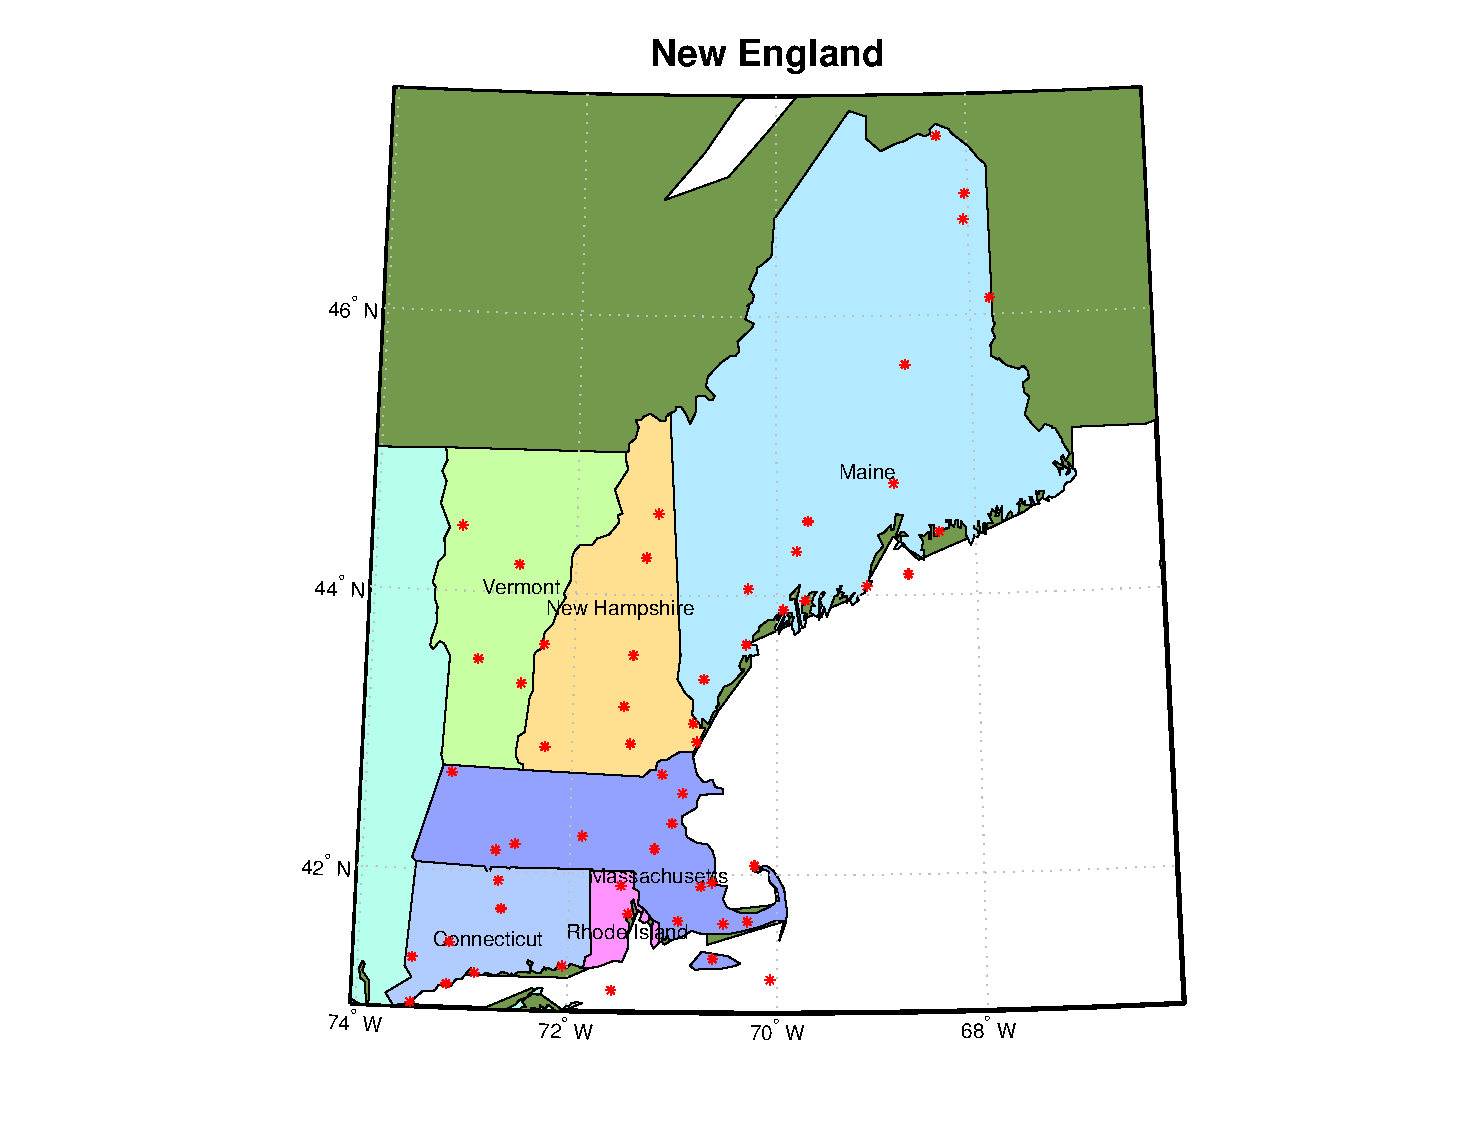
\includegraphics[width=\columnwidth]{img/NE_map}
\vspace{-0.35in}
\caption{Candidate locations in New England}
\label{fig:NE_locs}
\end{figure}

We adopt the values and approaches for computing PUE, datacenter
construction costs, wind farm construction costs, land costs,
transmission lines and network connection costs, and grid energy costs
from \cite{berral2014building}.  Table \ref{tab:loc-dependent-pars}
shows part of the location-dependent parameters for five sample
locations used in our experiments, and Table \ref{tab:constant-pars}
shows the values of the location-independent parameters.  Datacenter
construction costs are financed and amortized across 12 years.  Wind
farm construction costs are financed over 12 years and amortized over
24 years.  We assume that land cost is fully recoverable, so that the
only incurred cost is that of financing, spread over 12 years.
Finally, the cost for IT equipment is financed and amortized over 4
years.  For financing, we use an annual interest rate of 3.25\%.

\begin{table}[ht]
\begin{center}
\caption{Location-dependent parameter values for five sample
  locations.  %\thunote{Xiaoying, the maxPUE cannot possibly be that low, can it?}
  }
\begin{tabular}{|l|c|c|c|c|c|}
\hline
& \multicolumn{1}{p{22pt}|}{Burlinton, NH} &
\multicolumn{1}{p{28pt}|}{Springfield Hartnes, VT} &
\multicolumn{1}{p{20pt}|}{Nash Island, CT} &
\multicolumn{1}{p{27pt}|}{Marthas Vineyard, RI} &
\multicolumn{1}{p{27pt}|}{Mount Washington, NH}
\\
\hline
$pLand$ (\$/m$^2$)&946.9&946.9&946.9&680.21&946.9  \\
$maxPUE$&1.645&1.645&1.619&1.682&1.676 \\
$cLinePow$ (M\$)&64.5&77.2&16.6	&86.6&107.1 \\
$cLineNet$ (M\$)&13.5&16.7&16.9&17.7&21.3 \\
$pEnergy$ (\$/kWh)&0.0941&0.0941&0.1281&	0.1281&	0.1257 \\
Average $\beta$ (\%) &11.7&2.7&	40&	15.9&56.8 \\
\hline
\end{tabular}
\label{tab:loc-dependent-pars}
\end{center}
\vspace{-0.1in}
\end{table}

\begin{table}[ht]
\begin{center}
\caption{Values of location-independent parameters.}
\begin{tabular}{|l|c|c|}
\hline
\textbf{Parameter}& \textbf{Value} &\textbf{Unit}\\
\hline
$dcArea$ &	0.557& m$^2$/kW \\
$\textit{pBuildDC}$&12000& \$/kW	 \\
$serverPow$ 	&0.275&kW/serv \\
$switchPow$ 	&0.48 &kW/switch\\
$servsSwitch$ &	32 &servs/switch\\
$pServer$ 	&2000 &\$/serv\\
$pSwitch$  & 20000 &\$/switch\\
$\textit{pNBWServ}$&	1 & \$/serv-month\\
$wfArea$ &	18.21 & m$^2$/kW\\
$\textit{pBuildWF}$&	2.1& \$/kW \\

\hline
\end{tabular}
\label{tab:constant-pars}
\end{center}
\end{table}

We use the nominal grid load, which totals 6,254MW across all the
buses in the New England system.  For each time epoch $t$, we compute
the wind energy being generated by all the wind farms (existing ones
and the new one being placed) using $\beta(l,t)$.  We assume full
loading of all datacenters (existing ones and the new one being
placed).  We then compute the system loss for the time epoch for the
placement of the new datacenter and wind farm at locations $d$ and
$w$, respectively, using the simulation approach described in
Section~\ref{sec:quantify}.  We map the candidate locations in
Figure~\ref{fig:NE_locs} to buses using the approach previously
discussed in Section~\ref{sec:quantify}.  For each possible pair of
($d$, $w$), we sum the transmission loss over the entire year.
Finally, we set $pTransLoss$ to the maximum electricity price in the
whole area.

\subsubsection{Placement approaches}

As already discussed, the primary novelty of our optimization
framework is that it considers the cost of transmission system losses.
In addition, it also simultaneously places a new datacenter and an
offsetting wind farm.  To assess the impact of these characteristics,
we compare results for five different placement strategies as follows.

\textbf{DC\_WF\_OPT:} This strategy individually looks for the best
locations to put the datacenter and the wind farm; i.e., it solves the
optimization problem for the datacenter without considering the new
wind farm, and then solves the optimization problem again for the wind
farm without considering the new datacenter.  This strategy also
ignores transmission losses.  Note that assuming
a constant transmission loss would give the same results.

\textbf{DC+G\_WF+G:} This strategy is the same as DC\_WF\_OPT except
that grid transmission losses are considered when solving the optimization
problem.

\textbf{Min\_Loss:} This strategy finds locations for the datacenter
and wind farm that minimize the cost of transmission system losses.

\textbf{Co-location:} This strategy assumes that the datacenter and
wind farm should be co-located, and so finds a single location
that minimize the overall cost, including the cost of
the transmission system losses.

\textbf{Jointly:} This strategy considers the simultaneous placement
of the datacenter and wind farm, and uses all of the costs and
revenues in the optimization framework to find locations (the
datacenter and wind farm may be co-located or placed at different
locations) that minimize overall cost.

\subsubsection{Results}

Our results show that each placement strategy was able to find at
least one placement of the new datacenter and wind farm that satisfies
the constraints for avoiding the overloading of transmission lines and
unacceptable voltage variations throughout the simulated year.  This
is an important finding since overloading of transmission lines and
unacceptable voltage variations can have serious consequences as
already discussed.

Figure \ref{fig:cost1dc1wf} shows the resulting total cost when using
the five different placement strategies.  We observe that not
considering transmission system losses (DC\_WF\_OPT), considering only
transmission system losses (Min\_Loss), and forcing the co-location of
the datacenter and wind farm (Co-location) all lead to higher total cost.
Specifically, DC\_WF\_OPT incurs the highest transmission cost,
Min\_Loss incurs high cost for laying networking lines, and
Co-location incurs high energy cost.  In comparison, considering both
transmission system losses and datacenter construction/operation costs
can lead to finding locations that best balance these factors, leading
to lowest overall cost.

%\thunote{We cannot use this \$663M as the baseline.  Use the co-location as the baseline.}
The locations found and the total cost achieved by the five strategies
are listed in Table \ref{tab:costsaving}.  These results show that
using the full optimization framework (Jointly) achieves savings of
8\% compared to simply co-locating the datacenter and wind farm
(Co-location) and 3.4\% compared to not accounting for transmission
system losses (DC\_WF\_OPT).  Interestingly, the simultaneous
placement of datacenter and wind farm (Jointly) gives the same results
as the individual placement of datacenter and wind farm (DC+G\_WF+G).
Thus, our results do not provide evidence to support the importance of
simultaneous placement, and this issue should be studied further.  The
optimization problem can be solved more efficiently if we can view the
datacenter and wind farm placements as independent problems without
increasing the total cost.

\begin{figure}[ht]
\centering
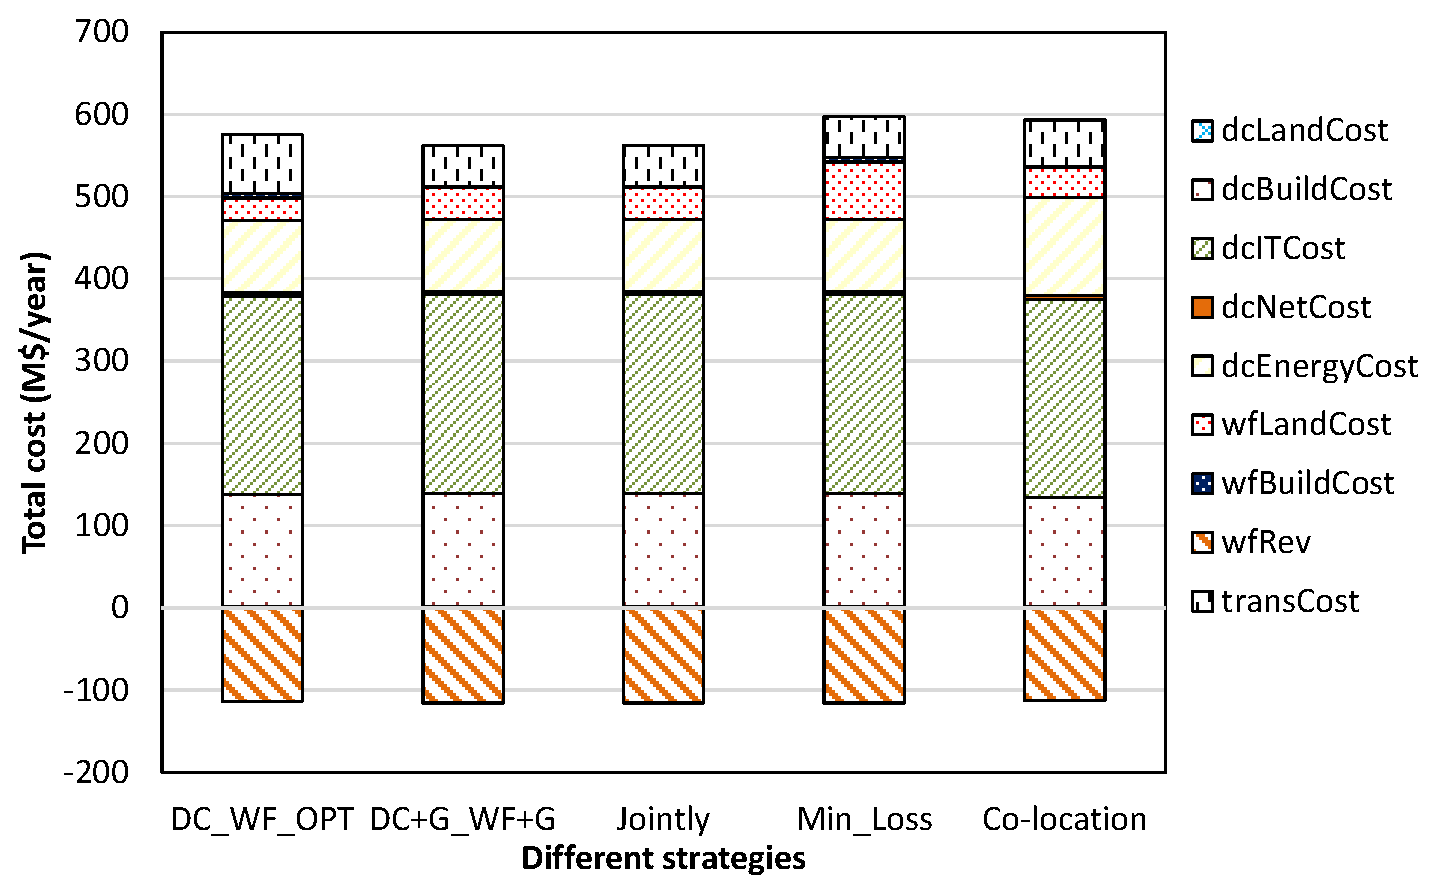
\includegraphics[width=1\columnwidth]{img/cost-one-dc-one-wf}
\caption{Cost of building/operating a 100MW datacenter and an offsetting wind farm.}
\label{fig:cost1dc1wf}
\end{figure}

\begin{table}[ht]
\begin{center}
\caption{Locations of datacenter and wind farm, and the resulting
  total costs.}
\begin{tabular}{|l|p{50pt}|p{50pt}|p{30pt}|p{20pt}|}
\hline
\textbf{Strategy}& \textbf{Datacenter location} &\textbf{Wind farm location} &\textbf{Total cost (M\$/year)}% & \textbf{Cost saving (\%)}
 \\
\hline
\textbf{DC\_WF\_OPT} &  Burlington,NH  & Mount Washington, NH & 461.5%& 30.4
\\
\textbf{DC+G\_WF+G} &Springfield Hartnes, VT  & Nash Island, CT& 446.2%& 32.7
\\
\textbf{Jointly} &Springfield Hartnes, VT&  Nash Island, CT & 446.2% & 32.7
\\
\textbf{Min\_Loss} &Springfield Hartnes, VT & Marthas Vineyard, RI & 481.5% & 27.4
\\
\textbf{Co-location}& Nash Island, CT &Nash Island, CT& 480.7% & 27.5
\\
\hline
\end{tabular}
\label{tab:costsaving}
\end{center}
\vspace{-0.2in}
\end{table}

%%% Local Variables:
%%% mode: latex
%%% TeX-master: "paper"
%%% End:
